\documentclass[conference]{IEEEtran} 

\usepackage[utf8x]{inputenc} 
\usepackage{graphicx}
\usepackage{mathtools, amsmath,amssymb}
\usepackage[ruled,vlined]{algorithm2e}
\usepackage{caption, subcaption}
\usepackage{todonotes}
\usepackage[para]{footmisc}
\usepackage{booktabs}
\usepackage{multirow}
\usepackage{xcolor,colortbl}
\usepackage{hyperref}
\usepackage{cleveref}
%\usepackage{mcite}
\usepackage[noadjust]{cite}

\def\BibTeX{{\rm B\kern-.05em{\sc i\kern-.025em b}\kern-.08em
    T\kern-.1667em\lower.7ex\hbox{E}\kern-.125emX}}
    
\begin{document} % 

\title{DeepCOVIDExplainer: Explainable COVID-19 Diagnosis from Chest X-ray Images}

\author{
\IEEEauthorblockN{
	Md. Rezaul Karim\IEEEauthorrefmark{1}\IEEEauthorrefmark{2},
	Till Döhmen\IEEEauthorrefmark{1}\IEEEauthorrefmark{2}, 
	Michael Cochez\IEEEauthorrefmark{3}, 
	Oya Beyan\IEEEauthorrefmark{1}\IEEEauthorrefmark{2},
	Dietrich Rebholz-Schuhmann\IEEEauthorrefmark{4},
	Stefan Decker\IEEEauthorrefmark{1}\IEEEauthorrefmark{2} 
}
    \IEEEauthorblockA{\IEEEauthorrefmark{1} Fraunhofer Institute for Applied Information Technology FIT, Germany}
    \IEEEauthorblockA{\IEEEauthorrefmark{2} Information Systems and Databases, RWTH Aachen University, Germany}
    \IEEEauthorblockA{\IEEEauthorrefmark{3} Information Center for Life Sciences~(ZB MED), German National Library of Medicine, Germany}
    \IEEEauthorblockA{\IEEEauthorrefmark{4} Department of Computer Science, Vrije Universiteit Amsterdam, the Netherlands}
}

\maketitle

\begin{abstract}
    %Amid the coronavirus disease~(COVID-19) pandemic, challenge hospitals are faced with, in the fight against the virus, is the effective screening of incoming patients.
    %One methodology is the assessment of  images, which usually requires expert radiologists' knowledge. 
    In this paper\footnote{Read longer version of this paper:~\url{https://arxiv.org/pdf/2004.04582.pdf}}, we propose an explainable deep neural networks~(DNN)-based method for automatic detection of COVID-19 symptoms from chest radiography~(CXR) images, which we call \emph{`DeepCOVIDExplainer'}. We used 15,959 CXR images of 15,854 patients, covering normal, pneumonia, and COVID-19 cases. CXR images are first comprehensively preprocessed and augmented before classifying with a neural ensemble method, followed by highlighting class-discriminating regions using gradient-guided class activation maps~(Grad-CAM++) and layer-wise relevance propagation~(LRP). Further, we provide human-interpretable explanations for the diagnosis. Evaluation results show that our approach can identify COVID-19 cases 
    %\footnote{Findings are not externally~(e.g., with radiologists/clinicians) validated yet.} 
    with a positive predictive value~(PPV) of 91.6\%, 92.45\%, and 96.12\%, respectively for normal, pneumonia, and COVID-19 cases, respectively, 
    %(and precision, recall, and F1 score of 94.6\%, 94.3\%, and 94.6\%, respectively)
    outperforming recent approaches. %We hope that our findings will be a useful contribution to the fight against COVID-19 and, in more general, towards an increasing acceptance and adoption of AI-assisted applications in the clinical practice.
\end{abstract}
\begin{IEEEkeywords} COVID-19, Biomedical imaging, Deep learning, Explainability, Grad-CAM, Layer-wise relevance propagation.\end{IEEEkeywords}

\section{Introduction}
\label{introduction}
The ongoing coronavirus pandemic%~(declared by the World Health Organization~(WHO) in March 2020) 
has already created a devastating impact on the health and well-being of the global population~\cite{wang2020covid,gozes2020rapid}. 
%As of November 6, 2020, it causes about 50 million infections of COVID-19 and 1.25 million fatalities\footnote{\url{https://www.worldometers.info/coronavirus/}}. 
Recent studies show that COVID-19, caused by severe acute respiratory syndrome coronavirus 2~(SARS-CoV-2), often, but by no means exclusively, affects elderly persons with pre-existing medical conditions~\cite{COVID1,COVID2,COVID3,huang2020clinical,ng2020imaging}.
%\footnote{List of abbreviations can be found in the end of this paper.}. 
While hospitals are struggling with scaling up capacities to meet the rising number of patients, it is crucial to make use of the screening methods at hand to identify COVID-19 cases and discriminate them from other conditions~\cite{wang2020covid}. 
The definitive test for COVID-19 is the reverse transcriptase-polymerase chain reaction~(RT-PCR) test, which requires specialized laboratories. COVID-19 patients, however, show several unique clinical and para-clinical features, e.g., presenting abnormalities in medical chest imaging with commonly bilateral involvement. Such features that are observable on CXR images and CT scans~\cite{huang2020clinical} are only moderately characteristic to the human eye~\cite{ng2020imaging} and not easy to distinguish from pneumonia. 

AI-based techniques have been utilized in numerous scenarios, including automated diagnoses and treatment in clinical settings. Deep neural networks~(DNNs) have been employed for the diagnosis of COVID-19 from medical images, leading to promising results~\cite{huang2020clinical,wang2020covid,ng2020imaging,ozturk2020automated,tabik2020covidgr}. However, many current approaches are ``black box" methods without providing insights into the decisive image features. 
Let's imagine a situation where resources are scarce, e.g., a hospital runs out of confirmatory tests or necessary radiologists are occupied, where AI-assisted tools could potentially help less-specialized general practitioners to triage patients, by highlighting critical chest regions to lead automated diagnosis decision~\cite{wang2020covid}. 

%A fully automated method without the possibility for human verification would, however, at the current state-of-the-art, be potentially dangerous in a practical setting. 
Although COVID-19 diagnosis approaches~\cite{COVID1,COVID2,narin2020automatic,wang2020covid,ozturk2020automated,karimdeepcovidexplainer,tabik2020covidgr} proposed recently looks promising when compared to expert radiologist a lower sensitivity in most of the cases, the reliability can be questioned for three main reasons. The datasets used are severely biased due to a deficient number of COVID-19 cases. Moreover, some results are not statistically reliable and lack of decision biases as the diagnoses were mostly based on a single model. Nevertheless, less accurate localization and visualization of critical chest regions.
%We hope that \emph{`DeepCOVIDExplainer'} will be a useful contribution towards the development and adoption of AI-assisted diagnosis applications in general, and for COVID-19 in particular. 
%To allow for the reproduction of results and derivative works, we will make the source code, documentation, and links to used data publicly available. 
%The rest of the paper is structured as follows: \Cref{sec:rw} outlines related works and points out potential limitations. \Cref{sec:mm} describes our proposed approach, before demonstrating experiment results in \cref{sec:er}. \Cref{sec:co} summarizes the work and provides some outlook before concluding the paper.
\iffalse
\section{Related Work}
\label{sec:rw}
Bullock et al.~\cite{bullock2020mapping} provides a comprehensive overview of recent application areas of AI against COVID-19, mentioning medical imaging for diagnoses first, which emphasizes the prevalence of the topic. Although PCR tests offer many advantages over CXR and CT~\cite{COVID3}, shipping the sample of patients is necessary, whereas X-ray or CT machines are readily available even in rather remote areas. In a recent study by K. Lee et al.~\cite{COVID1}, CXR and CT images from nine COVID-19 infected patients were analyzed by two radiologists to assess the correspondence of abnormal findings on X-rays with those on CT images. The proportion of patients with abnormal initial radiographic findings was 78.3\% to 82.4\% for SARS and 83.6\% for MERS, while being only 33\% for COVID-19 cases~\cite{COVID1}. 
Chest CT images, in contrast, showed double lung involvement in eight out of nine patients. In other words, X-ray may not be the best imaging method for detecting COVID-19, judging by the small cohort of nine patients~\cite{COVID1}. Another study by Yicheng Fang et al.~\cite{COVID2}, however, supports those findings and argues in favor of the effectiveness of CT over X-ray. CT should hence cautiously be considered as the primary imaging source for COVID-19 detection in epidemic areas~\cite{COVID3}. %Nevertheless, the limited patient cohort size leaves room for statistical variability and, in contrast to those findings, a few other studies have reported rather promising results for the diagnosis based on CXR imaging~\cite{wang2020covid,narin2020automatic,ghoshal2020estimating}.

Narin et al. \cite{narin2020automatic} evaluated different convolutional neural networks~(CNN) for the diagnosis of COVID-19 and achieved an accuracy of 98\% using a pre-trained ResNet50 model. However, the classification problem is overly simplified by only discriminating between healthy and COVID-19 patients, disregarding the difficulty of distinguishing regular pneumonia conditions from COVID-19 conditions.  
Wang et al. \cite{wang2020covid} proposed COVID-Net to detect distinctive abnormalities in CXR images among samples of patients with non-COVID-19 viral infections, bacterial infections, and healthy patients. 
On a test sample of 92 positive COVID-19 cases among approx. 300 other cases, COVID-Net reaches an overall accuracy of 92.6\% with 97.0\%, 90.0 \%, and 87.1 \% sensitivity for normal, Non-COVID-19, and COVID-19 cases, respectively. 
%On the other hand, COVID-Net achieves PPV of 90.5\%, 91.3\%, and 98.9\% for normal, Non-COVID-19, and COVID-19 cases, respectively. 
%Still, the small sample size does not enable generalizable statements about the reliability of the method. Highlighted regions using `GSInquire' are also not well-localized to critical areas. 
%Overall, training on imbalance data, lack of thorough image preprocessing, and poor decision visualization have hindered this approach. 

Ozturk et al.~\cite{ozturk2020automated} proposed DarkCovidNet to provide automatic diagnosis of COVID-19 based on CXR images. Trained on only 125 CXR images DarkCovidNet model to provide COVID-19 diagnosis in two ways: i) binary classification showing COVID-19 vs no-findings and multiclass classification showing COVID-19 vs no-findings vs pneumonia, giving an accuracy of 98.08\% and 87.02\%, 
%for binary and multiclass classification settings, 
respectively. %Although the end-to-end COVID-19 diagnostic pipeline is very comprehensive and backed by `you only look once'~(YOLO) real-time object detection system, it has two potential limitations, including a severely low number of image samples and imprecise localization on the chest region. 
Biraja G. et al. \cite{ghoshal2020estimating} employed uncertainty estimation and interpretability based on the Bayesian approach to CXR-based COVID-19 diagnosis, which shows interesting results. The results may, however, be impaired by a lack of appropriate image preprocessing and the resulting attention maps show somewhat imprecise areas of interest. Tabik et al.~\cite{tabik2020covidgr} curated a richer dataset called COVIDGR-1.0 containing 377 positive and 377 negative postero anterior CXR views, reaching  
%They subsequently, proposed COVID Smart Data based Network~(aka. COVID-SDNet). 
%As claimed, their approach reaches 
an accuracy of 97.37\%$±$1.86\%,88.14\%$±$2.02\%, 66.5\%$±$8.04\% in severe, moderate, and mild COVID severity levels. 

Although these results look promising when compared to expert radiologist sensitivity of 69\%~\cite{tabik2020covidgr}, in most of the cases, the reliability can be questioned for three main reasons. The datasets used are severely biased due to a deficient number of COVID-19 cases~\cite{tabik2020covidgr}. Secondly, some results are not statistically reliable and lack of decision biases as the diagnoses were mostly based on a single model. Thirdly, less accurate localization and visualization of critical chest regions.
\fi 
To overcome the shortcomings and as a quick step towards an AI-based COVID-19 diagnosis, we propose \emph{`DeepCOVIDExplainer'}, a novel diagnosis approach based on neural ensemble method. 
%our approach first enriches existing datasets with more COVID-19 samples, followed by a comprehensive preprocessing pipeline for CXR images and data augmentation.
Based on the following hypotheses, DeepCOVIDExplainer focuses on fairness, algorithmic transparency, and explainability:

\begin{itemize}
    \item Based on majority voting from a panel of independent radiologists~(i.e., ensemble), we get the final prediction fair and trustworthy than a single radiologist.
    \item By localizing class-discriminating regions with Grad-CAM++ and LRP, we not only can mitigate the opaqueness of the black-box model by providing more human-interpretable explanations of the predictions, but also identify the critical regions on patients chest.
\end{itemize}

\section{Methods}
\label{sec:mm}
The pipeline of DeepCOVIDExplainer starts a comprehensive preprocessing of CXR images, followed by training of DenseNet, ResNet, and VGGNet architectures, and creating respective model snapshots. To incorporate the trained model into an ensemble, both Softmax class posterior averaging~(SCPA) and prediction maximization~(PM) are utilized. Finally, class-discriminating attention maps are generated using Grad-CAM++ and LRP to provide explanations and to identify critical regions on patients chest.

\subsection{Preprocessing}
Since radiographs usually have dark edges, images with such distinctly darker regions impact the  classification~\cite{86}). 
%We perform necessary preprocessing steps so that the model not only learns to identify black pixels in edges and to improve the generalization. 
We perform global contrast enhancement, edge enhancement, and noise elimination on entire CXR images with histogram equalization and unsharp masking edge enhancement. %Since , we perform the  of CXR images using HGE. 

\iffalse
By merging gray-levels with low frequencies into one, stretching high frequent intensities over high range of gray levels, HGE achieves close to equally distributed intensities~\cite{90}, where the probability density function $p(X_{k})$ of an image $X$ is defined as~\cite{90}:

%\vspace{-2mm}
\begin{equation}
\scriptsize{
    p(X_{k})=\frac{n_{k}}{N},}
    \label{eq3.1}
\end{equation}
%\vspace{-2mm}

\noindent where $k$ is the grey-level ID of an input image $X$ varying from 0 to $L$, $n_{k}$ is the frequency of a grey level $X_{k}$ in $X$, and $N$ is the number of images. 
%A plot of $n_{k}$ vs. $X_{k}$ is specified as the histogram of $X$, while the 
The equalization transform function $f(X_{k})$ is tightly related to cumulative density function~\cite{90}:

%\vspace{-2mm}
\begin{equation}
\scriptsize{
    f(X_{k})=X_{0}+(X_{L}-X_{0})c(X_{k}) \\
    c(X_{k})=\sum_{j=0}^{k}p(X_{j}).}
\end{equation}
%\vspace{-2mm}

\noindent Output of HGE, $Y={Y(i,j)}$ is synthesized as follows~\cite{90}:

%\vspace{-2mm}
\begin{equation}
\scriptsize{
    Y=f(X)=\left\{f(X(i,j))|\forall X(i,j) \in X\right\}.}
\end{equation}  

\iffalse
\vspace{-2mm}
\begin{figure*}
	\centering
	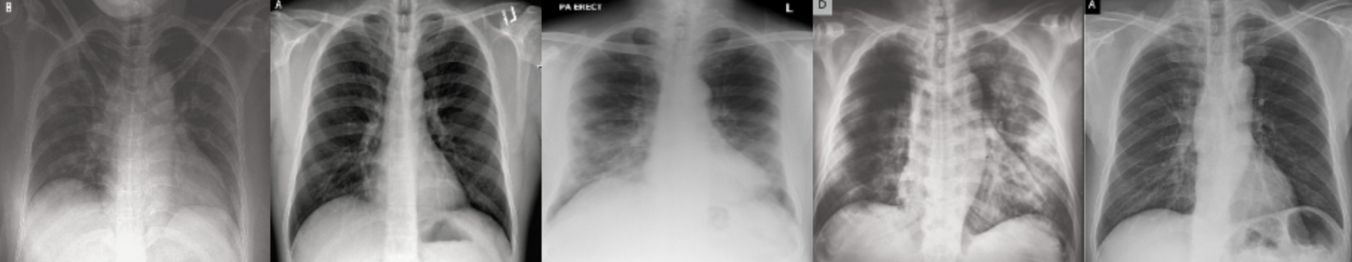
\includegraphics[width=0.9\textwidth,height=20mm]{covix.png}	
    \caption{Sample CXR from COVIDx dataset showing COVID-19 confirmed cases}	
	\label{fig:viz2}
	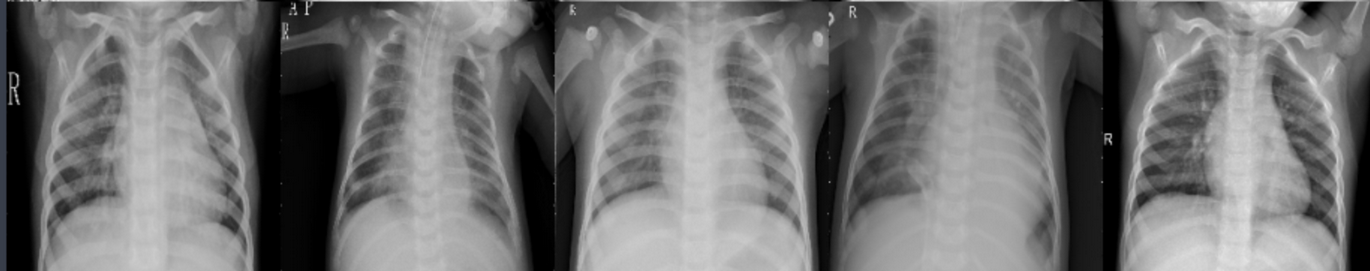
\includegraphics[width=0.9\textwidth,height=20mm]{kg.png}	
    \caption{Sample CXR images from RSNA Pneumonia Detection Challenge}	
	\label{fig:viz}
\end{figure*}
\vspace{-2mm}
\fi 

\vspace{2mm}
Image filters `edge enhances' and `sharpen' are adopted with the convolution matrices as kernel $g(.)$. PMF is used to preserve the edges and detailed structures along with noise reduction as long as the fitting diffusion coefficient $c(.)$ and gradient threshold $K$ are separate~\cite{95}. As a non-linear anisotropic diffusion model, PMF smoothens noisy images $\theta (x,y)$ w.r.t. partial derivative as~\cite{95}:

\vspace{-2mm}
\begin{equation}
\scriptsize{
    \frac{\partial u}{\partial t}= div(c(|\nabla u(x,y,t)|)\nabla u(x,y,t)),}
\end{equation}
\vspace{-2mm}

\noindent  where $u(x,y,0)$ is the original image, $\theta (x,y)$, $u(x,y,t)$ is a filtered image after $t$ iteration diffusion; $div$ and $\nabla$ are divergence and gradient operators w.r.t spatial variables $x$ and $y$, where the diffusion coefficient $c(.)$ is computed as~\cite{96}:

\vspace{-2mm}
\begin{equation}
\scriptsize{
    c_{1}(|\nabla I|)=exp \left(- \left(\frac{|\nabla I|}{K} \right)^{2} \right)} 
\end{equation}
%\vspace{-2mm}

\vspace{-4mm}
\begin{equation}
\scriptsize{
    c_{2}(|\nabla I|)=\frac{1}{1+\left(\frac{|\nabla I|}{K} \right)^{2}}. }
\end{equation}
%\vspace{-2mm}

To check local gradient magnitudes can preserve edges, updated diffusion coefficient function is computed~\cite{96}: 

%\vspace{-2mm}
\begin{equation}
\scriptsize{
    c_{3}(|\nabla I|)=\left\{
    \begin{array}{lr}
    \frac{1}{2}\left[1-\left(\frac{|\nabla I|}{K\sqrt{2}}\right)^{2}\right]^{2}, &|\nabla I|\leq K\sqrt{2}\\
    0,& |\nabla I|> K\sqrt{2}
    \end{array}
    \right.}
    \label{eq3.9}
\end{equation}
%\vspace{-2mm}

\noindent where $c_{3}$ is the Tukey's biweight function. Since the boundary between noise and edge is minimal, $c_{3}$ is applied as the fitting diffusion coefficient~\cite{95}. Further, we attempt to remove textual artifacts from CXR images, e.g., a large number of images annotate right and left sides of the chest with a white `R' and `L' characters. We threshold the images first to remove very bright pixels and the missing regions were in-painted. In other scenarios, image standardization and normalization are performed. 
%Mean pixel values are subtracted from each pixel and divided by the standard deviation of all pixel values. 
%The mean and standard deviation is calculated on the whole datasets and adopted for training, validation, and test sets. 
Further, CXR images are resized $224 \times 224 \times 3$ before starting the training and rescaled pixel values to a [0,1] by using a pixel-wise multiplication factor of 1/255. %, giving a collection of grey-scale images. 

\begin{figure*}
	\centering
	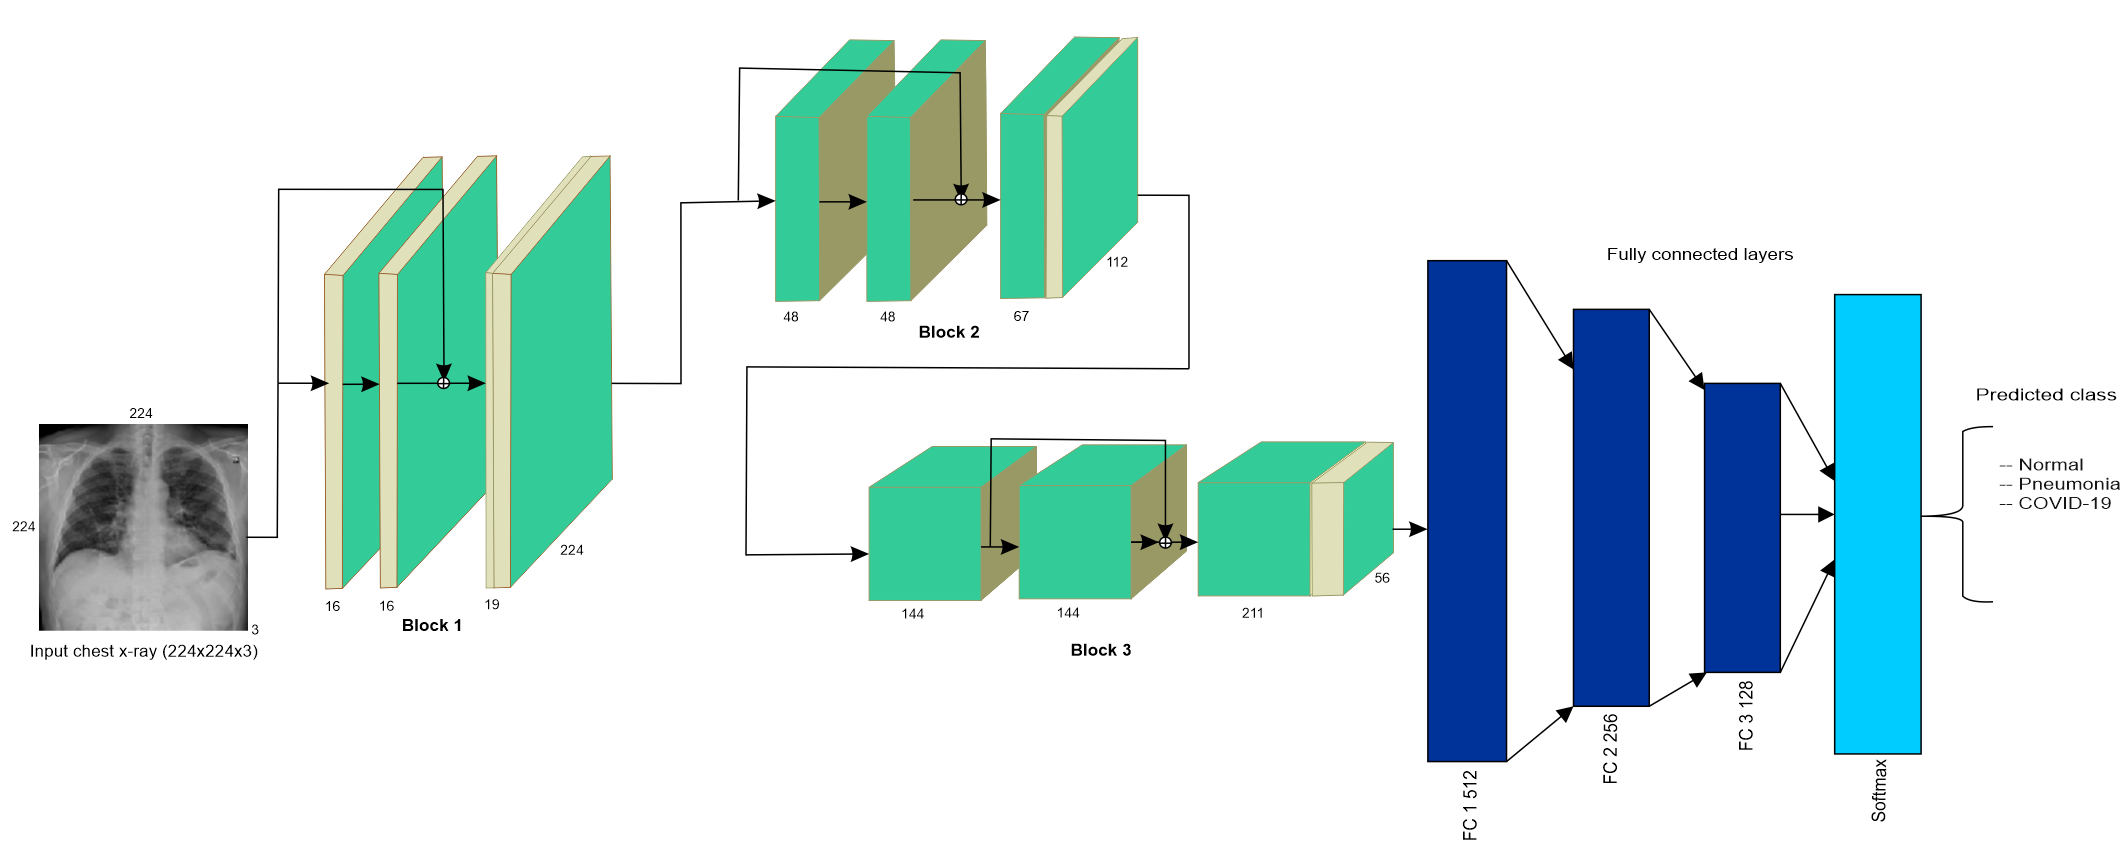
\includegraphics[width=0.9\linewidth,height=70mm]{densenet.png}
	\caption{The classification with ResNet-based networks} 
	\label{fig:resnet}
\end{figure*}
\fi

\begin{figure*}[h]
	\centering
	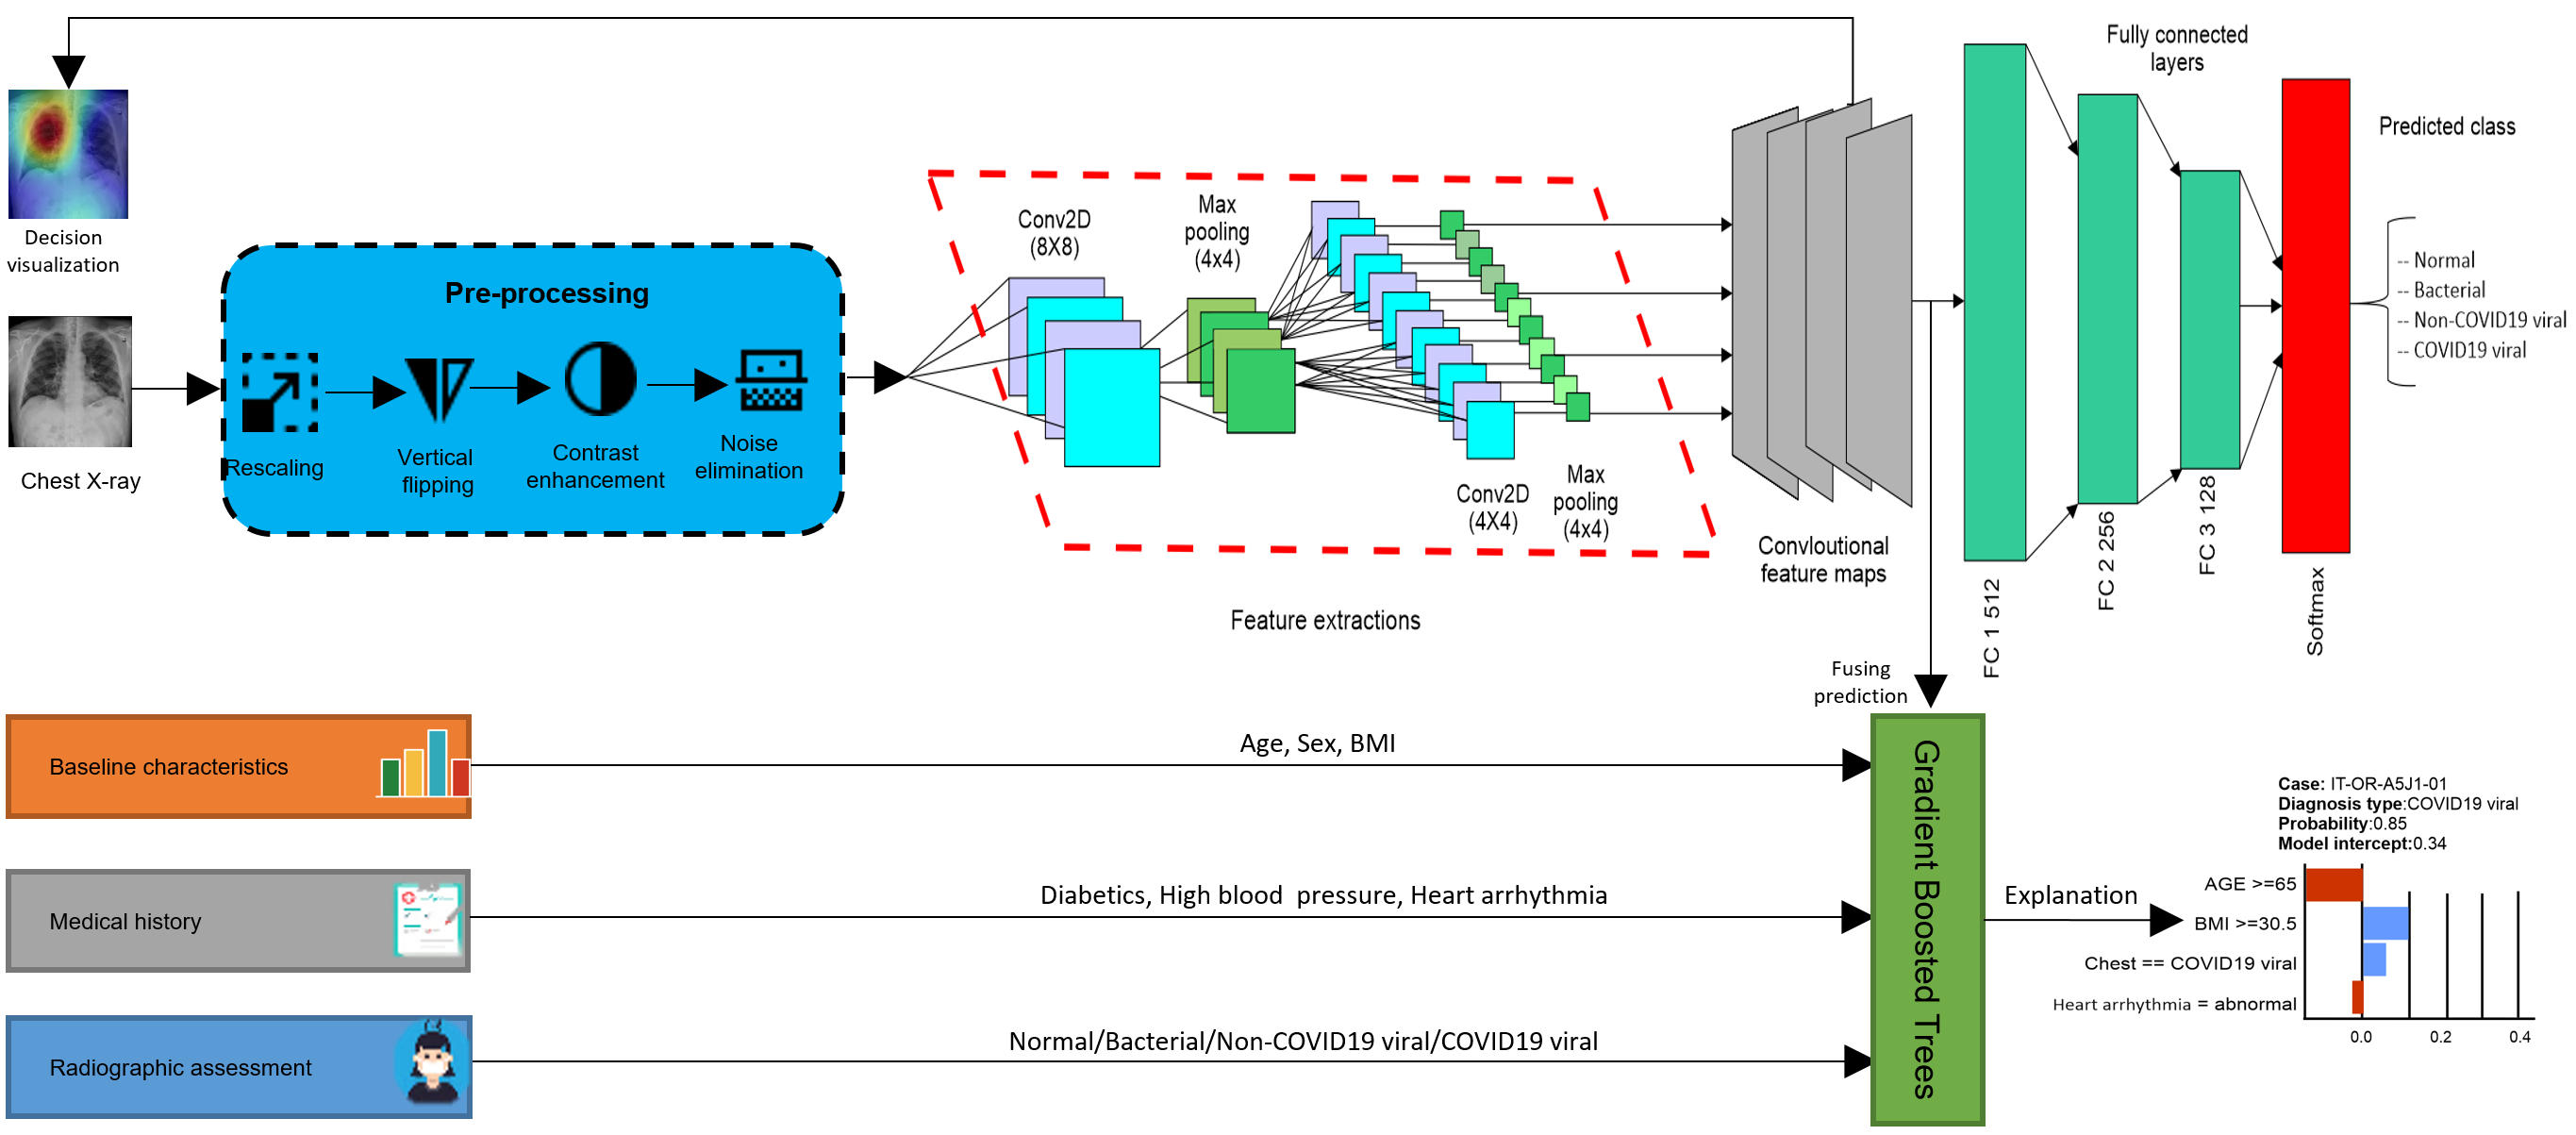
\includegraphics[width=0.8\textwidth,height=45mm]{wf.png}
    \caption{Classification and decision visualization with CNN-based approach}	
	\label{fig:viz}
	\vspace{-2mm}
\end{figure*}

\subsection{Network construction and training}
We train VGG-16/19, ResNet-18/34, and DenseNet-161/201 architectures and create their snapshots during a single run with cyclic cosine annealing~(CAC)%~(see \cref{fig:cac})
\cite{loshchilov2016sgdr}, followed by combining their predictions to an ensemble prediction~\cite{huang2017snapshot,karim2019snapshot}. 
%We pick VGG-16 and VGG-19 due to their general suitability for image classification. 
%Based on the dense evaluation concept~\cite{108}, VGG variants convert the last three fully connected layers~(FCLs) to 2D convolution operations to reduce the number of hyperparameters. We keep last 2 layers fixed to adopt a 1$\times$1 kernel, leaving the final one equipped with a Softmax activation. 
%However, %owing to the computational complexity of VGG-16 due to consecutive FCLs, 
%the revised VGG-19 is trained with a reduced number of hidden nodes in the first 2 FCLs.
%Besides we pick ResNet-18 and ResNet-34~\cite{106},  
%ResNets are lightweight stack-based CNNs, with their simplicity arising from small filter sizes~(i.e., 3$\times$3)~\cite{108}. Apart from common building blocks, two bottlenecks are present in the form of channel reduction. % in ResNets. 
%A series of convolution operators without pooling is placed in between, forming a stack. The first conv layer of each stack in ResNets~(except for the first stack) are down-sampled at stride 2, which provokes the channel difference between identity and residual mappings. 
%A series of convolution operators without pooling is placed in between and recognized as a stack. %, as shown in \cref{fig:resnet}.
%However, w.r.t regularisation, a 7$\times$7 conv filter is decomposed into a stack of three 3$\times$3 filters with non-linearity injected in between~\cite{108}. 
%DenseNet-161, and DenseNet-201 architectures to concatenate additional inputs from preceding layers. 
%, while ResNets merge feature-maps through summation. 
%It strengthens feature propagation and moderates information loss and increases feature reusing capability by reducing numbers of parameters~\cite{109}.  
%\FloatBarrier
\iffalse
\begin{figure*}
    \centering
    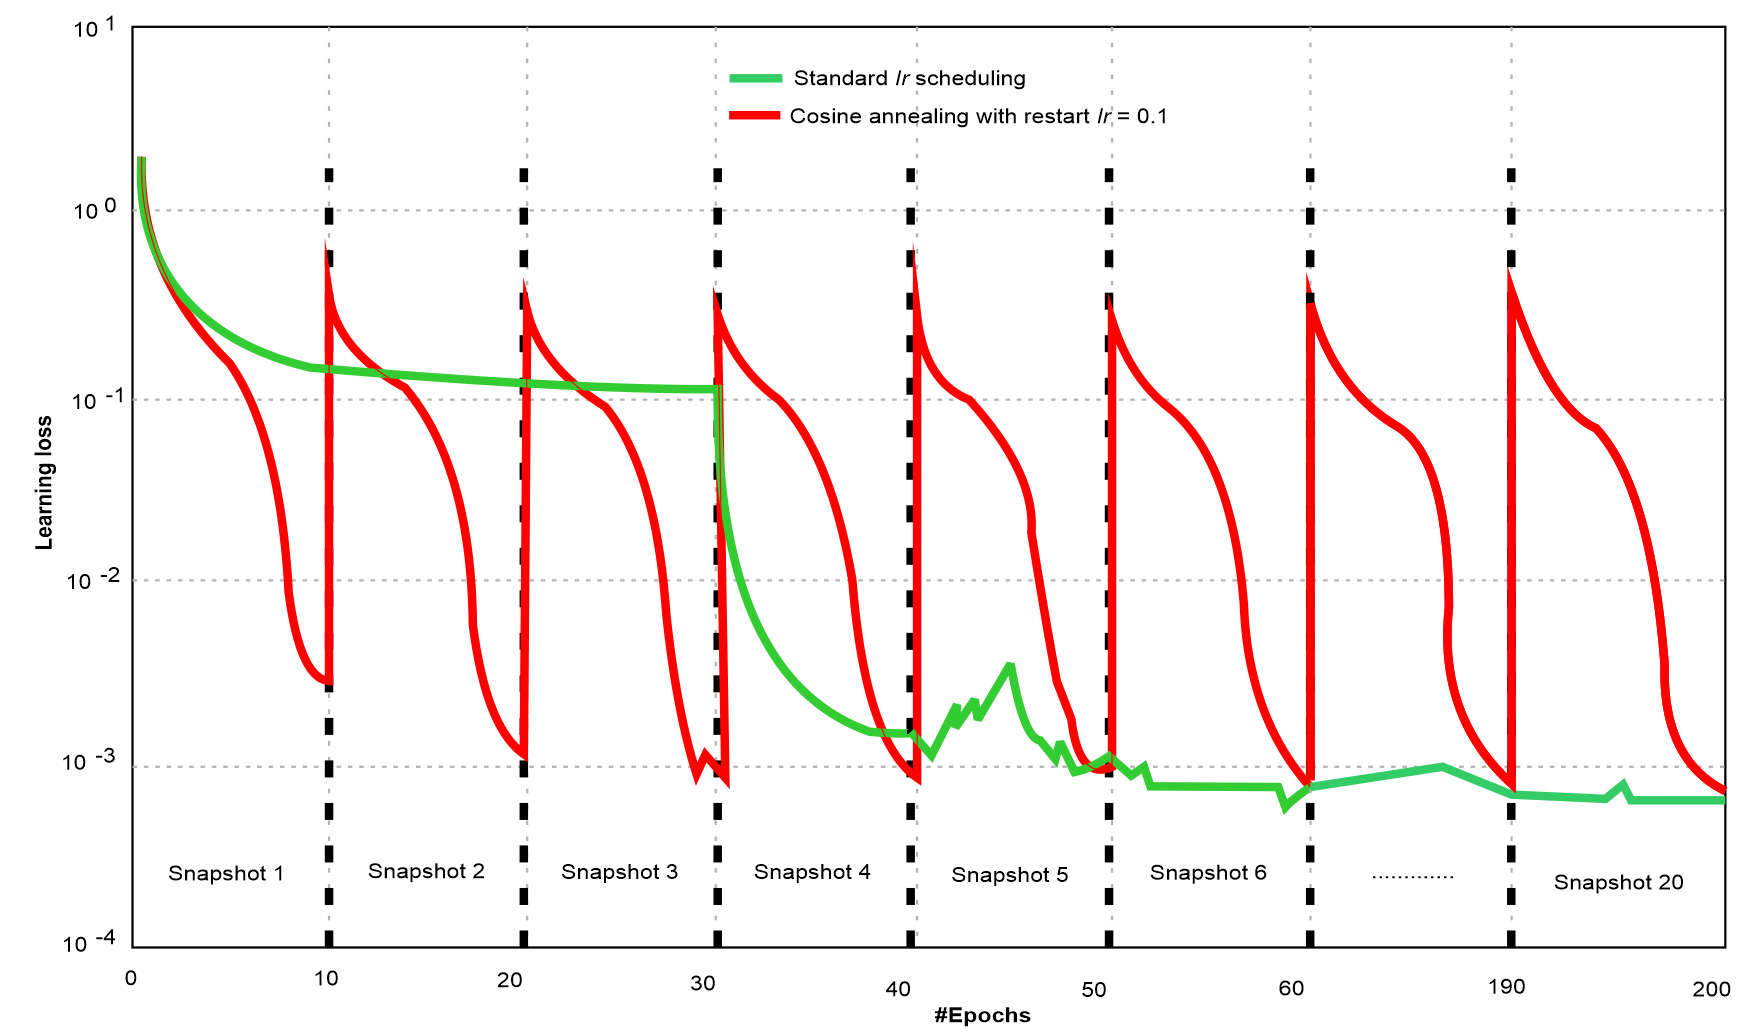
\includegraphics[width=0.8\textwidth,height=70mm]{ca.png}
    \caption{Training loss of VGG-19 network with standard learning rate~(green) and cosine annealing cycles~(red), the intermediate models, denoted by the dotted lines form an ensemble at the end of training}
    \label{fig:cac}
\end{figure*}
\fi
%To avoid possible overfitting, $L_2$ weight regularization, dropout, and data augmentation
%~(by rotating CXR images by up to 15$^\circ$) 
%were employed. 
We do not initialize network weights with pretrained~(as general object like shapes are not present in CXR images~\cite{karimdeepcovidexplainer}) models. We set number of epochs~(NE), learning rate~(LR), number of cycles~(NC), and current epoch number. CAC starts with a large LR and rapidly decreases to a minimum value before it dramatically increases systematically over epochs to produce different network weights~\cite{huang2017snapshot}: 

\vspace{-2mm}
\begin{equation}
    \label{eq:lr-cosine}
    \scriptsize{
    \alpha(t)=\frac{\alpha_{0}}{2}\left(\cos \left(\frac{\pi \bmod (t-1,\lceil T / C\rceil)}{\lceil T / C\rceil}\right)+1\right),}
\end{equation}

where $\alpha(t)$ is the LR at epoch $t$, $\alpha_0$ is the maximum LR, $T$ is the total epoch, $C$ is the number of cycles and $mod$ is the modulo operation. After training a network for $C$ cycles, best weights at the bottom of each cycle are saved as a model snapshot~($m$), giving $M$ model snapshots, where $m \leq M$. 

\subsection{Model ensemble}
When a single radiologist makes a COVID-19 diagnosis, the chance of a false diagnosis is high. Therefore, it is reasonable to ask for a second or third opinions. %Analogous to this principle, 
We employ neural ensemble to combine the `expertise' of multiple models into a consolidated prediction~\cite{huang2017snapshot}, as neural ensemble method by combining several deep architectures is more effective than structures solely based on a single model~\cite{huang2017snapshot,karim2019snapshot}. 
We apply both SCPA and PM of best-performing snapshot models, ensemble their predictions, and propagate them through the Softmax layer, where the class probability of the ground truth $j$ for a given image $x$ is inferred as~\cite{7}:

\vspace{-2mm}
\begin{equation}
\scriptsize{
    P(y=j | \mathbf{x})=\frac{\exp \left[\sum_{m=1}^{M} \hat{P}_{m}(y=j | \mathbf{x})\right]}{\exp \left[\sum_{k=1}^{K} \sum_{m=1}^{M} \hat{P}_{m}(y=k | \mathbf{x})\right]},}
\end{equation}

where $m$ is the last snapshot model from $M$, $K$ is the number classes, and $\hat{P}_{m}(y=j | \mathbf{x})$ is the probability distribution. 

\subsection{Decision visualizations}
To improve diagnosis transparency, critical chest regions are localized with Grad-CAM~\cite{114}, Grad-CAM++~\cite{chattopadhay2018grad}, and LRP~\cite{LRP2}. The idea is to explain where the model provides more attention for the classification in terms of heatmaps, 
%for all the test samples are generated based on the trained models, 
indicating the relevance for the classification decision.

\iffalse
CAM computes the number of weights of each feature map~(FM) based on the final conv layer to calculate the contribution to prediction $y_c$ at location $(i,j)$, where the goal is to obtain $L_{ij}^{c}$ that satisfies $y^{c}=\sum_{i, j} L_{ij}^{c}$. The last FM $A_{ijk}$ and the prediction $y_c$ are represented in a linear relationship in which linear layers consist of global average pooling~(GAP) and FCLs: i) GAP outputs $F_{k}=\sum_{i,j} A^k_{ij}$, ii) FCL that holds weight $w_{k}^{c}$, generates the following output~\cite{kim2020extending}: 
 
 %\vspace{-2mm}
 \begin{equation}
 \scriptsize{
     y^{c}=\sum_{k} w_{k}^{c} F_{k}=\sum_{k} w_{k}^{c} \sum_{i,j} A^k_{ij}=\sum_{i, j} \sum_{k} w_{k}^{c} A^k_{ij},}
 \end{equation}
 %\vspace{-2mm}
 
where $A^{k}$ represents the visualization of the $k^{th}$ feature map, $L_{i j}^{c}=\sum_{k} w_{k}^{c} A^k_{ij}$~\cite{kim2020extending}. Due to the vanishing of non-linearity of classifiers, CAM is an unsuitable method. Hence, we employ Grad-CAM to globally average the gradients of FM as weights instead of pooling, while class-specific weights are collected from the final conv layer through globally averaged gradients~(GAG) of FM instead of pooling~\cite{chattopadhay2018grad}: 

%\vspace{-2mm}
\begin{equation}
\scriptsize{
    \alpha_k^c=\frac{1}{Z}\sum_{i}\sum_{j}\frac{\partial y^c}{\partial A_{ij}^k},}
    \label{eq:alpha}
\end{equation}
%\vspace{-2mm}

where $Z$ is the number of pixels in an FM, $c$ is the gradient of the class, and $A_{ij}^k$ is the value of $k^{th}$ FM. Having gathered relative weights, the coarse saliency map~(SM), $L^c$ is computed as the weighted sum of $\alpha_k^c*A_{ij}^k$ of the ReLU activation.
It introduces linear combination to the FM as only the features with a positive influence on the respective class are of interest~\cite{chattopadhay2018grad} and the negative pixels that belong to other categories in the image are discarded~\cite{114}:

\vspace{-2mm}
\begin{equation}
\scriptsize{
    L^c=\operatorname{ReLU}(\sum_{i}\alpha_k^cA^k),}
    \label{3.11}
\end{equation}
\vspace{-4mm}

Grad-CAM++~(see \cref{fig:viz}) replaces the GAG with a weighted average of the pixel-wise gradients as the weights of pixels contribute to the final prediction w.r.t the following iterators over the same activation map $A^k$, $(i,j)$ and $(a,b)$: 

\vspace{-2mm}
\begin{equation}
\scriptsize{
    w_k^c=\sum_{i}\sum_{j}\alpha_{ij}^{kc}\cdot \operatorname{ReLU}(\frac{\partial y^c}{\partial A_{ij}^k})}
\end{equation}
\vspace{-2mm}

\begin{equation}
\scriptsize{
    y^c=\sum_{k}w_k^c\cdot \sum_{i}\sum_{j}A_{ij}^k.} 
\end{equation}
\vspace{-4mm}

\begin{equation}
\scriptsize{
    \alpha_{ij}^{kc}=\frac{\frac{\partial^2y^c}{(\partial A_{ij}^k)^2}}{2\frac{\partial^2y^c}{(\partial A_{ij}^k)^2}+\sum_{a}\sum_{b}A_{ab}^k{\frac{\partial^3y^c}{\{(\partial A_{ij}^k)^3\}}}}.}
    \label{eq:w}
\end{equation}
\vspace{-2mm}

Even though CXR images rarely contain multiple targets, revealing particular image parts that contributed to the prediction, rather than entire chest area is still helpful. CAM variants that back-propagate the gradients all the way up to the inputs, are essentially propagated only till the final conv layer. Besides, CAM methods are limited to specific architectures, where an average-pooling layer connects conv layers with an FCL. LRP is another technique for propagating relevance scores~(RS). In contrast to CAM, LRP redistributes proportionally to the activation of previous layers. LRP assumes that the class likelihood can be traced backwards through a network to the individual layer-wise nodes of the input~\cite{LRP2}. From a network of $L$ layers, $1,2,...,N$ nodes in layer $l$, $1,2,..,M$ nodes in layer $l+1$, the RS, $R_{n}^{(l)}$ at node $n$ in layer $l$ is recursively defined as follows~\cite{LRP2}:   
%\vspace{-2mm}
\begin{equation}
\scriptsize{
    R_{n}^{(l)}=\sum_{m} \frac{a_{n}^{(l)} w_{n, m}^{+(l)}}{\sum_{n^{\prime}} a_{n^{\prime}}^{(l)} w_{n^{\prime}, m}^{+(l)}} R_{m}^{(l+1)}.}
\end{equation}
\vspace{-2mm}

The node-level RS for negative values is calculated with ReLU activation function as follows~\cite{LRP2}:

\vspace{-2mm}
\begin{equation}
\scriptsize{
    R_{n}^{(l)}=\sum_{m} \frac{x_{n}^{(l)} w_{n, m}^{(l)}-b_{n}^{(l)} w_{n, m}^{+(l)}-h_{n}^{(l)} w_{n, m}^{-(l)}}{\sum_{n^{\prime}} x_{n^{\prime}}^{(l)} w_{n^{\prime}, m}^{(l)}-b_{n^{\prime}}^{(l)} w_{n^{\prime}, m}^{+(l)}-h_{n^{\prime}}^{(l)} w_{n^{\prime}, m}^{-(l+1)}}.}
\end{equation}
\vspace{-2mm}

\noindent Output layer RS is calculated before  back-propagating~\cite{LRP2}:

\vspace{-2mm}
\begin{equation}
\scriptsize{
    R_{n}^{(L)}=\left\{\begin{array}{ll}
    {z_{t}^{(L)}} & {n=t} \\
    {0} & {\text {otherwise.}}
    \end{array}\right.}
\end{equation}
\vspace{-2mm}

First, an image $x$ is classified in a forward pass, where LRP identifies important pixels. The backward pass is a conservative relevance~(i.e., $R_{t}^{(L)}$) redistribution procedure with back-propagation using deep Taylor decomposition~\cite{DTD}, to generate a relevance map $R_{lrp}$, for which the nodes contributing most to the higher-layer, also receive most relevance. 
\fi 
 % for each.

\section{Experiments}
\label{sec:er}
%In this section, we discuss our evaluation results both quantitative and qualitatively, showing a comparative analysis. %\subsection{Experiment setup}
%Experiments were carried out on a machine having an Intel(R) Xeon(R) E5-2640, 256 GB of RAM, and Ubuntu 16.04 OS. 
%Methods\footnote{\url{https://github.com/BioXAI/DeepCOVIDExplainer}} were written in Python with scikit-learn and Keras. % with the TensorFlow backend. 
%The LRP-based visualization and relevance calculation are generated using the iNNvestigate toolbox\footnote{\url{https://github.com/albermax/innvestigate}}.
%Networks were trained on an Nvidia Titan Xp GPU. % with CUDA. %, and cuDNN enabled to make the overall pipeline faster. 
During the training\footnote{Source code: \url{https://github.com/rezacsedu/DeepCOVIDExplainer}}, we set the NE to 200, maximum LR to 1.0, and NC to 20, giving 20 snapshots for each model and 120 snapshot models in total, on which we construct the ensemble model. The best snapshot model, which is used for the decision visualizations is chosen using WeightWatcher~\cite{martin2019traditional}. 
%To tackle the class imbalance issue, we apply class weighting to penalize a model when it misclassifies a positive sample. 
%Although accuracy is an intuitive evaluation criterion for many bio-imaging problems, e.g., osteoarthritis severity prediction, those evaluation criteria are most suitable for balanced class scenarios. Keeping in mind the imbalanced scenario with widely different class distributions between classes,
%We report precision, recall, F1, and positive predictive value~(PPV). % produced through random search and 5-fold cross-validation tests. %, i.e., for each hyperparameter group of the specific network structure, 5 repeated experiments are conducted.

\subsection{Datasets}
\label{sec:ds}
%We consider 2 different versions of the datasets: first, we used the \emph{`COVIDx v1.0'} dataset by Wang et al.~\cite{wang2020covid} used to train and evaluate the COVID-Net, comprised of a total of 13,975 CXR images across 13,870 patient cases\footnote{As of June 6, 2020}. COVIDx is mainly based on RSNA Pneumonia Detection Challenge\footnote{\url{https://www.kaggle.com/c/rsna-pneumonia-detection-challenge}}, ActualMed COVID-19 Chest X-ray Dataset Initiative\footnote{\url{https://github.com/agchung/Figure1-COVID-chestxray-dataset}}, COVID-19 radiography database\footnote{\url{https://www.kaggle.com/tawsifurrahman/covid19-radiography-database}}, 

%giving 219 COVID-19 positive images, 1,341 normal images, and 1,345 viral pneuomonia images. This gives 358 CXR images from 266 COVID-19 patient cases and total of 8,066 patient cases who have no pneumonia~(i.e., normal) and 5,538 patient cases who have non-COVID19 pneumonia. 
%had a total of 5,941 CXR images from 2,839 patients based on the COVID-19 image dataset curated by Joseph P., et al.~\cite{cohen2020covid} and Kaggle CXR Pneumonia dataset\footnote{\url{https://www.kaggle.com/paultimothymooney/chest-xray-pneumonia}} by Paul Mooney. It is used in some early works, e.g.,~\cite{wang2020covid}. However, Kaggle CXR images are of children. 
%Therefore, to avoid possible prediction bias~(e.g., the model might be prone to predict based on mere chest size), 
The updated dataset~\footnote{Refer to \url{https://github.com/rezacsedu/DeepCOVIDExplainer} for the detail.}, which we refer to \emph{`COVIDx v2.0'} is categorized as normal~(i.e., no-findings), pneumonia, and COVID-19 viral are enriched with CXR images of adult subjects of COVID-19, pneumonia, and normal examples, leaving 15,959 CXR images across 15,854 patients: 

\iffalse
\vspace{1mm}
\begin{itemize}%[noitemsep]
    \item {COVID chest X-ray-dataset}: Joseph P.C. et al.~\cite{cohen2020covid}\footnote{\url{https://github.com/ieee8023/covid-chestxray-dataset}}: 660 PA~(i.e., frontal view) CXR images. 
    \item {COVID-19 patients lungs X-ray images}\footnote{\url{https://www.kaggle.com/nabeelsajid917/covid-19-x-ray-10000-image}}: 70 COVID-19 and 70 normal CXR images. 
    \item {Chest X-ray images} by Ozturk et al.~\cite{ozturk2020automated} \footnote{\url{https://github.com/muhammedtalo/COVID-19}}: 125 COVID-19, 500 normal, and 500 pneumonia CXR images. 
\end{itemize}
\vspace{1mm}
%\Cref{tab:train_test_dist} and \cref{Tab:class_dist} show the  distributions of class, images, and patients.
\fi 

\iffalse
\begin{table}
	\centering
	\caption{Train and test set distribution in COVIDx datasets}
	\label{tab:train_test_dist}
	\begin{tabular}{p{2.5cm}|p{1.5cm}|p{1.5cm}}
		\hline
		\textbf{COVIDx version} & \textbf{Training}& \textbf{Test}\\	
		\hline
		v1.0 & 5,344 & 654\\
		\hline
		v2.0 & 11,744 & 5,032\\
		\hline
		v3.0 & 11,896 & 5,099\\
		\hline
	\end{tabular}
\end{table} 
\begin{table}
	\centering
	\caption{The class distribution of COVIDx datasets}
	\label{Tab:class_dist}
	%\scriptsize{
	\begin{tabular}{p{0.9cm}|p{1cm}|p{1.1cm}|p{2cm}|p{1.1cm}p{0.5cm}}
	\hline
	\textbf{Version}& \textbf{Normal}& \textbf{Bacterial} & \textbf{Non-CoVID19 viral}& \textbf{COVID-19} \\
		\hline 
		v1.0 & 1,583 & 2,786 & 1,504 & 76\\
		\hline
		\textbf{Version}& \textbf{Normal}& \multicolumn{2}{c|}{\textbf{Pneumonia}}  &  \textbf{COVID-19}\\	
		\hline
		v2.0 & 8,066 & \multicolumn{2}{c|}{8,614} & 190\\
		\hline
		v3.0 & 8,066 & \multicolumn{2}{c|}{8,614} & 259\\
		\hline
	\end{tabular}
	%}
\end{table} 
\fi 

\subsection{Performance of individual model}
As summarized in \cref{Table:all_models}, VGG-19 and DenseNet-161 performed best on both balanced and imbalanced datasets, albeit %, while VGG-16 turns out to be the least performing.
i) VGG-19 outperforms VGG-16, and ii) %, which can be explained by the fact that a classifier with more formations requires more fitting of FMs, which again depends on conv layers. 
%The architecture modification of VGG-19 by setting 2 conv layers and the filter size of 16, visibly enhances the performance. 
ResNet-18 performed better than ResNet-34. %, although it's larger counterpart ResNet-34 shows very unexpected low performance. %Evidently, due to structured residual blocks, the accumulation of layers could not promote FMs extracted from the CXR images.
\begin{table*}
    \centering
	\caption{Classification results of each model on balanced and imbalanced datasets} 
	\label{Table:all_models}
	%\vspace{-4mm}
	\scriptsize{
	\begin{tabular}{p{2.9cm}p{1.6cm}p{1.4cm}p{1.0cm}p{0.3cm}p{1.5cm}p{1.4cm}p{1.0cm}}
	 & \multicolumn{3}{c}{\bfseries{Balanced dataset}} && \multicolumn{3}{c}{\bfseries{Imbalanced dataset}} \\
		\cmidrule{2-4}\cmidrule{6-8}   
        \textbf{Network}& \textbf{Precision} & \textbf{Recall}& \textbf{F1} && \textbf{Precision} & \textbf{Recall}& \textbf{F1}\\
		\hline
		VGG-16 & 0.783 & 0.771 & 0.761 && 0.734 & 0.753 & 0.737\\
		ResNet-34 & 0.884 & 0.856 & 0.861 && \textbf{0.852} & \textbf{0.871} & \textbf{0.851} \\
		DenseNet-201  & 0.916 & 0.905 & 0.905 && 0.805 & 0.773 & 0.826\\		
		ResNet-18 & 0.924 & 0.925 & 0.921 && 0.873 & 0.847 & 0.852\\
		VGG-19 & \textbf{0.943} & \textbf{0.935} & \textbf{0.925} && 0.862 & 0.848 & 0.845\\
		DenseNet-161  & \textbf{0.952} & \textbf{0.945} & \textbf{0.948} && \textbf{0.893} & \textbf{0.874} & \textbf{0.883}\\
		\hline
	\end{tabular}}
	\vspace{-2mm} 
\end{table*}
DenseNet-161 outperforms other models, giving precision, recall, and F1 scores of 0.952, 0.945, and 0.945, respectively, on balanced CXR images. %VGG-19 also gives a comparable performance, giving precision, recall, and F1 scores of 0.943, 0.935, and 0.939, respectively. 
On imbalanced dataset, both DenseNet-161 and ResNet-18 perform consistently. Although VGG-19 and ResNet-18 show competitive results on balanced dataset, the misclassification rate for normal and pneumonia samples are slightly elevated than DenseNet-161, which poses a risk for clinical diagnosis. 
While DenseNet-161 is found to be resilient against class imbalanced, making it better suited for the clinical setting. %, where COVID-19 cases are rare compared to pneumonia or normal cases. %The ROC curve of DenseNet-161 model in \cref{fig:rocs} shows consistent AUC scores across folds, indicating not only stable predictions but also better prediction than random guessing. 
%Nevertheless, lousy snapshot models can contaminate the overall predictive powers of the ensemble model. Hence, we use WeightWatcher to choose the best model. First, we choose top-5 snapshots to generate a full model and choose top-3 models for the final ensemble model. then, we compare top models
%~(by excluding VGG-16, ResNet-34, and DenseNet-201) 
%and choose the ones with the lowest log norm and highest weighted alpha, where a low log-norm signifies better generalization of network weights~\cite{martin2019traditional}. %, %. \Cref{fig:weight_watch} shows choosing the better model between VGG-16 and VGG-19 with WeightWatcher 
%in terms of weighted alpha and log norm.

%\FloatBarrier
\subsection{Model ensemble}
\label{model_ensemble}
We perform the ensemble on following top-3 models: VGG-19, ResNet-18, and DenseNet-161. %To ensure a variation of network architectures within the ensemble, VGG-19 is also included. 
As demonstrated in \cref{Table:ensemble_result}, the ensemble based on the SCPA method moderately outperforms the ensemble based on the PM method. The reason is that the PM approach appears to be easily influenced by outliers with high scores. %To a great extent, the mean probabilities for each class affect the direction of outliers. 
For the SCPA-based ensemble, the combination of VGG-19 + DenseNet-161 outperforms other ensemble combinations. Results show that a majority of samples were classified correctly, with precision, recall, and F1 scores of 0.937, 0.926, and 0.931, respectively, using the PM ensemble method.
%The confusion matrix of the best ensemble's performance on balanced data is shown in \cref{fig:conf}. 
The SCPA-based ensemble yields slightly higher precision, recall, and F1 of 0.946, 0.943, and 0.945, respectively. We report the class-specific measures in \cref{Table:class_specific_result}. % to provide a better view in both balanced and imbalanced scenarios.

\begin{table*}
    \centering
    \caption{Classification results for ensemble methods on balanced dataset}
	\label{Table:ensemble_result}
	%\vspace{-4mm}
	\scriptsize{
	\begin{tabular}{p{4.3cm}p{1.6cm}p{1.1cm}p{0.8cm}p{0.1cm}p{1.6cm}p{1.1cm}p{0.8cm}}
		 &  \multicolumn{3}{c}{\textbf{Prediction maximization}} && \multicolumn{3}{c}{\textbf{Softmax posterior averaging}}  \\	
		\cmidrule{2-4}\cmidrule{6-8}
		\textbf{Architecture combination} &  \textbf{Precision} & \textbf{Recall}& \textbf{F1}&& \textbf{Precision} & \textbf{Recall}& \textbf{F1}\\
		\hline
		ResNet-18+DenseNet-161 & 0.915 & 0.924 & 0.928 && 0.925 & 0.94 & 0.933\\
		VGG-19+DenseNet-161 & \textbf{0.937} & \textbf{0.926} & \textbf{0.931} && \textbf{0.946} & \textbf{0.943} & \textbf{0.945}\\
		VGG-19+ResNet-18 & 0.917 & 0.923 & 0.912 &&  0.923 & 0.945 & 0.934\\
		DenseNet-161+VGG-19+ResNet-18 & 0.926 & 0.901 & 0.901 && 0.924 & 0.937 & 0.935\\
		\hline 
	\end{tabular}}
	\vspace{-2mm}
\end{table*}

\subsection{Quantitative analysis}
Since we primarily want to limit the number of missed COVID-19 instances, a recall of 90.5\% is still an acceptable metric compared to 91\% by Wang et al.~\cite{wang2020covid}.
%, i.e., a certain fraction of all patients who test positive, will actually not have the disease. 
To determine how many of all infected persons would be diagnosed positively, we calculate the PPV, where out of 129 COVID-19 samples, only 3 were misclassified as pneumonia and two as normal, giving a PPV of 96.12\% for COVID-19 cases. This is still an acceptable metric compared to 98.9\% by Wang et al.~\cite{wang2020covid}. 
%Besides, to provide a direct comparison, our approach slightly outperforms COVID-Net~\cite{wang2020covid} w.r.t normal vs. non-COVID19 cases. 

%Further, to provide a one-to-one comparison with COVID-Net, we further apply similar techniques on the \emph{`COVIDx v1.0'} dataset. The evaluation result was carried out on a test set of 92 COVID-19 cases, only 3 were misclassified as pneumonia, resulting in a PPV of 96.74\% for COVID-19 cases. This is, however, slightly lower than that of COVID-Net. However, we would still argue that it is an acceptable metric compared to 98.9\% by Wang et al.~\cite{wang2020covid}. 
%It is important to note that PPV was reported for a low prevalence of COVID-19 in the cohorts. 
In a setting with high COVID-19 prevalence, the likelihood of false-positives is expected to reduce in favor of correct COVID-19 predictions. Our results are backed up by i) a larger test set, ii) better localization and explanation capability, which contributes to the reliability of our evaluation results, given the fact that in healthcare predicting something with high confidence only is not enough, but requires trustworthiness. 

\begin{table*}
    \centering
	\caption{Classwise classification results of ensemble model on chest x-rays}
	\label{Table:class_specific_result}
	%\vspace{-4mm}
	\begin{tabular}{p{3.2cm}p{1.7cm}p{1.1cm}p{1.3cm}p{0.1cm}p{1.7cm}p{1.2cm}p{1.0cm}}
		 & \multicolumn{3}{c}{\textbf{Balanced dataset}} && \multicolumn{3}{c}{\textbf{Imbalanced dataset}} \\	
		\cmidrule{2-4}\cmidrule{6-8}
		\textbf{Infection type} & \textbf{Precision} & \textbf{Recall}& \textbf{F1}&& \textbf{Precision} & \textbf{Recall}& \textbf{F1}\\	
		\hline
		Normal & 0.942 & 0.927 & 0.935 && 0.906 & 0.897 & 0.902\\
		Pneumonia & 0.916 & 0.928 & 0.922 && 0.864 & 0.853 & 0.858\\
		COVID-19 & 0.904 & 0.905 & 0.905 && 0.877 & 0.881 & 0.879\\
		\hline
	\end{tabular}
	\vspace{-2mm}
\end{table*}

\begin{figure*}
	\centering
    	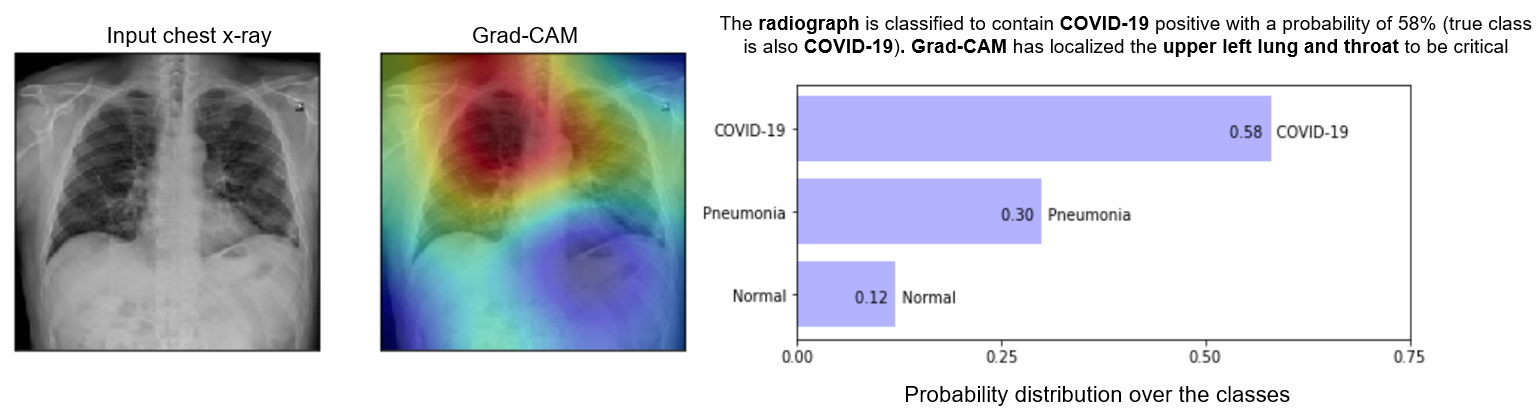
\includegraphics[width=0.7\textwidth,height=30mm]{samples/gradcam_1.png}
    	\caption{Classification of CXR with DenseNet-161, decision visualization with Grad-CAM, \& human-interpretable explanation}
    	\label{Fig:ggcam_viz}
    	\smallskip
    	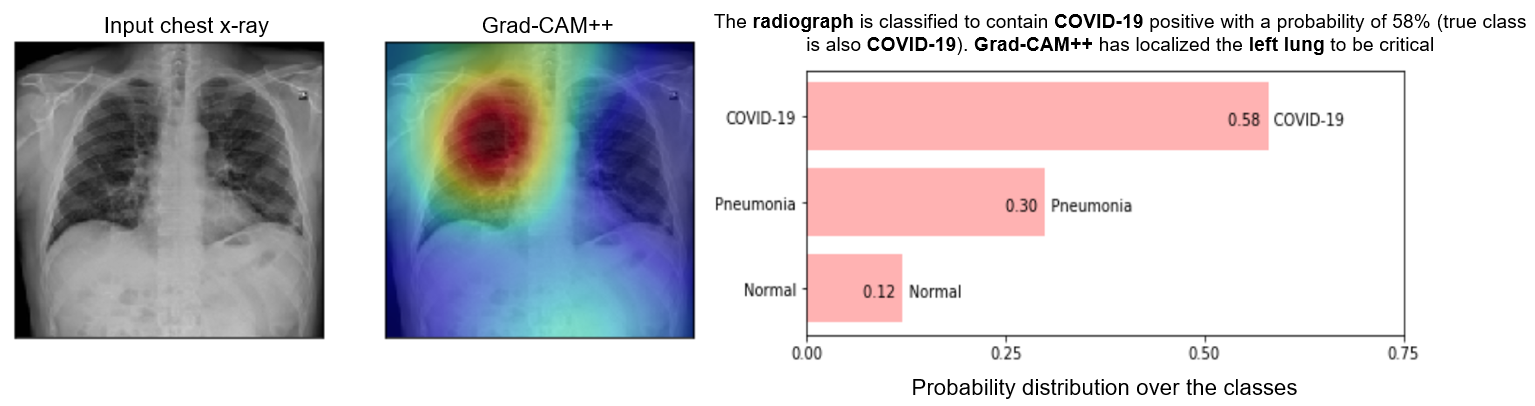
\includegraphics[width=0.7\textwidth,height=30mm]{samples/gradcam++_1.png}
    	\caption{Classification of CXR with DenseNet-161, decision visualization with Grad-CAM++, \& human-interpretable explanation}
    	\label{Fig:ggcam_plus_viz}
    	\smallskip
    	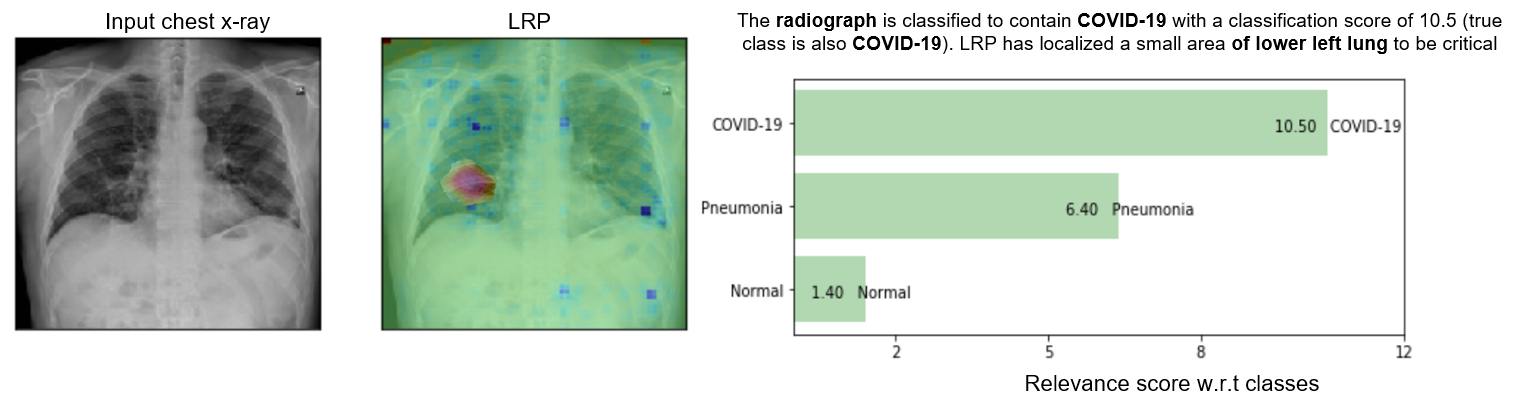
\includegraphics[width=0.7\textwidth,height=30mm]{samples/lrp1.png}
    	\caption{Classification of CXR with DenseNet-161, decision visualization with LRP, and human-interpretable explanation}
    	\label{Fig:lrp_viz}
    	\vspace{-2mm}
\end{figure*}

\subsection{COVID-19 predictions and explanations}
\label{sub:expl}
%Precise decisive feature localization is vital not only for the explanation but also for rapid confirmation of the reliability of outcomes, especially for potentially false-positive cases \cite{chattopadhay2018grad}. Attention map highlighting of critical regions on the chest advocate transparency and trustworthiness to clinicians and help them leverage their screening skills to make faster and yet more accurate diagnoses \cite{wang2020covid}. 
%In general, the more accurate a model is, the more consistent the visualizations of Grad-CAM and Grad-CAM++ will be. Key features can then easily be identified based on where the activation maps are overlapping. 

Critical regions of some CXR images of COVID-19 cases are highlighted in \cref{Fig:ggcam_viz}, \cref{Fig:ggcam_plus_viz}, and \cref{Fig:lrp_viz}, where class-discriminating areas within the lung are localized.
%\vspace{-2mm}
As seen, HM generated by Grad-CAM and Grad-CAM++ are fairly consistent and alike, but those with Grad-CAM++ are more accurately localized, i.e., instead of certain parts, Grad-CAM++ highlights conjoined features more precisely.
Although LRP highlights regions much more precisely, it fails to provide attention to critical regions. It turned out that Grad-CAM++ generates the most reliable HM when compared to Grad-CAM and LRP. Let's consider the following examples: 

%\vspace{-2mm}
\begin{itemize}
    \item \textbf{Example 1}: CXR image is classified to contain a confirmed COVID-19 case with a probability of 58\%, the true class is COVID-19, as shown in \cref{Fig:ggcam_viz}. 
    \item \textbf{Example 2}: CXR image is classified to contain a confirmed COVID-19 case with a probability of 58\%, the true class is COVID-19, as shown in \cref{Fig:ggcam_plus_viz}. 
    \item \textbf{Example 3}: CXR image is classified to contain COVID-19 case with a classification score of 10.5, the true class is COVID-19, as shown in \cref{Fig:lrp_viz}.
\end{itemize}

\subsection{Discussion and diagnosis recommendations}
%Based on the above analyses, \emph{`DeepCOVIDExplainer'} disseminates the following recommendations: 
Even if a specific approach does not perform well, an ensemble of several models still may outperform individual models. However, models trained on imbalanced training data may provide distorted or wrong predictions. In this case, even a high accuracy score can be achieved without predicting minor classes, hence might be uninformative. 
Thirdly, the risk resulting from a pneumonia diagnosis is much lower than for a COVID-19 diagnosis. Hence, it is more reasonable to make a decision based on the maximum score from individual model predictions. Fourthly, decision visualizations cannot be provided based on ensemble models, albeit their usage contributes to decision reliability. Therefore, it is recommended to pick the single best model as a basis and to employ Grad-CAM++ for providing the most reliable localization. 

%\newpage

\section{Conclusion and Outlook}
\label{sec:co}
In this paper, we proposed \emph{`DeepCOVIDExplainer'} to leverage explainable COVID-19 prediction based on CXR images. Evaluation results show that our approach can identify COVID-19 with a PPV of 96.12\% and recall of 94.3\%, outperforming a recent approach. 
However, since as Curtis Langlotz\footnote{\url{https://www.nature.com/articles/d41586-019-03847-z}} stated ``AI won't replace radiologists, but radiologists who use AI will replace radiologists who don't''. 
We would argue \emph{`DeepCOVIDExplainer'} 
%to be evaluated in a clinical setting, 
with no means a replacement for a human radiologist. 
%In contrast, human judgment is indispensable when the life of patients is at stake. 
%Further, we hope our findings will be a useful contribution to the fight against COVID-19 and towards an increasing acceptance and adoption of AI-assisted applications in the clinical practice. 
%Lastly, we want to outline potential areas of improvements: first, 
On a serious note: due to limited number of CXR images used to train the models, it would be unfair to claim that we can rule out overfitting for our models. 
%More unseen data from similar distributions are necessary for trustworthy diagnoses. 
%to avoid possible out-of-distribution issues. 
Besides, we were yet not been able to verify the diagnoses and localization accuracies with the radiologists. 
%Thirdly, accurate predictions not only depend on single imaging modalities but could also build upon additional modalities like CT and other decisive factors like patients' demographic and symptomatic assessment report. %~\cite{7}. 
%Although, explaining predictions with plots and charts are useful for exploration and discovery, communicating them to patients may be tedious and require more human-interpretable decision rules in natural language. 
In the future, we intend to overcome these limitations with a multimodal learning~(CT scans, CXR, and clinical notes) outcomes.

\bibliographystyle{IEEEtran}
\bibliography{sample-base.bib}

\end{document}